\chapter{Testing \& Evaluation} \label{cha:testing}
\section{Using the System}
To test Aims and Objectives 1 \& 2, \todo{finish this section}

for All tests in this section a Raspberry Pi 4b was used to host client code, running Raspberry Pi OS Lite (with no desktop environment), which was released on December 11th 2023. The server and frontend were hosted on a Laptop with an Intel i5-12450H processor, running Fedora 39 Linux. The Raspberry Pi's hostname (visible in screenshots) is "nikpi".
\subsection{Controlling one connected device} 
Perhaps the most obvious and basic test is to create a device, using the Rust client library, have it run on a device and to connect with that device to a running server. 

\subsubsection{Testing Setup}
A simple client was created, with two capabilities "Turn On" and "Turn Off". The callback functions attached to these capabilities would simply log to the standard output the name of the capability they are attached to. The Raspberry Pi is connected to the same Wi-Fi network as the server. The port 2302 has opened on the laptop's firewall to ensure the Raspberry Pi can make requests to the gRPC server. The Raspberry Pi is being controlled through a secure shell connection (SSH) (visible on the left side of screenshots). View figure~\ref{fig:example_config_raspi} for the exact configuration of the client.
\begin{figure}[h]
\caption{Client's configuration file}
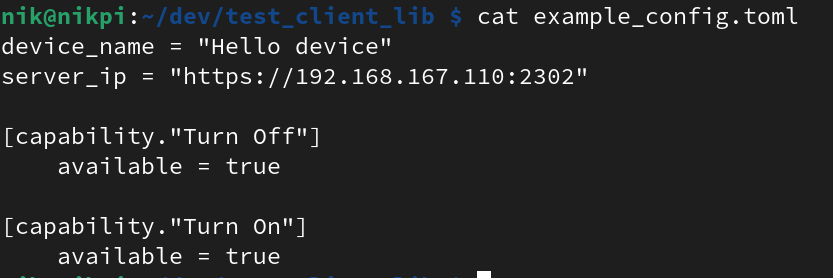
\includegraphics[width=\textwidth]{example_config_raspi}
\label{fig:example_config_raspi}
\end{figure}

\subsubsection{Testing}
Figure~\ref{fig:establish_connection_raspi} shows the successful connection and certificate exchange between the client on nikpi and the server. Note that the server ip that the client is connecting to is set within the client's configuration file (view figure~\ref{fig:example_config_raspi}). In this case the server (on the right side of figure~\ref{fig:establish_connection_raspi}) is being started with the "json-frontend" flag, as discussed within subsection~\ref{sec:chapimpl:frontend:json}, this flag is required to use the web-based frontend.
\begin{figure}[h]
\caption{Establishing a connection }
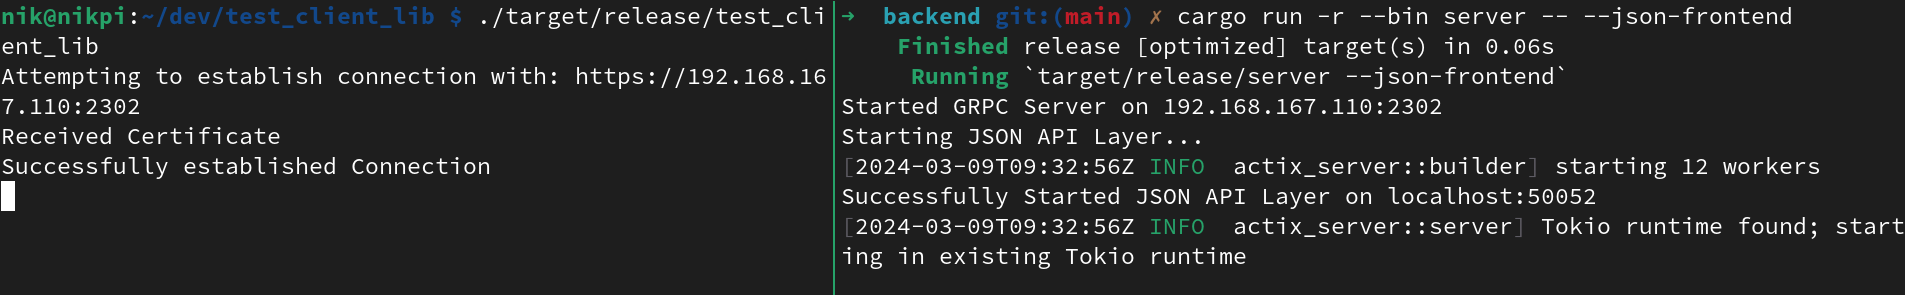
\includegraphics[width=\textwidth]{establish_connection_raspi}
\label{fig:establish_connection_raspi}
\end{figure}

The next important test is viewing the web frontend, to see that the device is correctly displayed on the frontend, with the appropriate capabilities. This can be seen in figure~\ref{fig:web_frontend_one_connected_device}, where the device, named "Hello device" (view configuration file) can be seen with it's two capabilities "Turn Off" and "Turn On". The web-frontend is being hosted by a Vite server, through using the command "npm run dev", on localhost port 5173. The frontend is being displayed by the Chromium web browser.
\begin{figure}[h]
\caption{Web Frontend with the connected device}
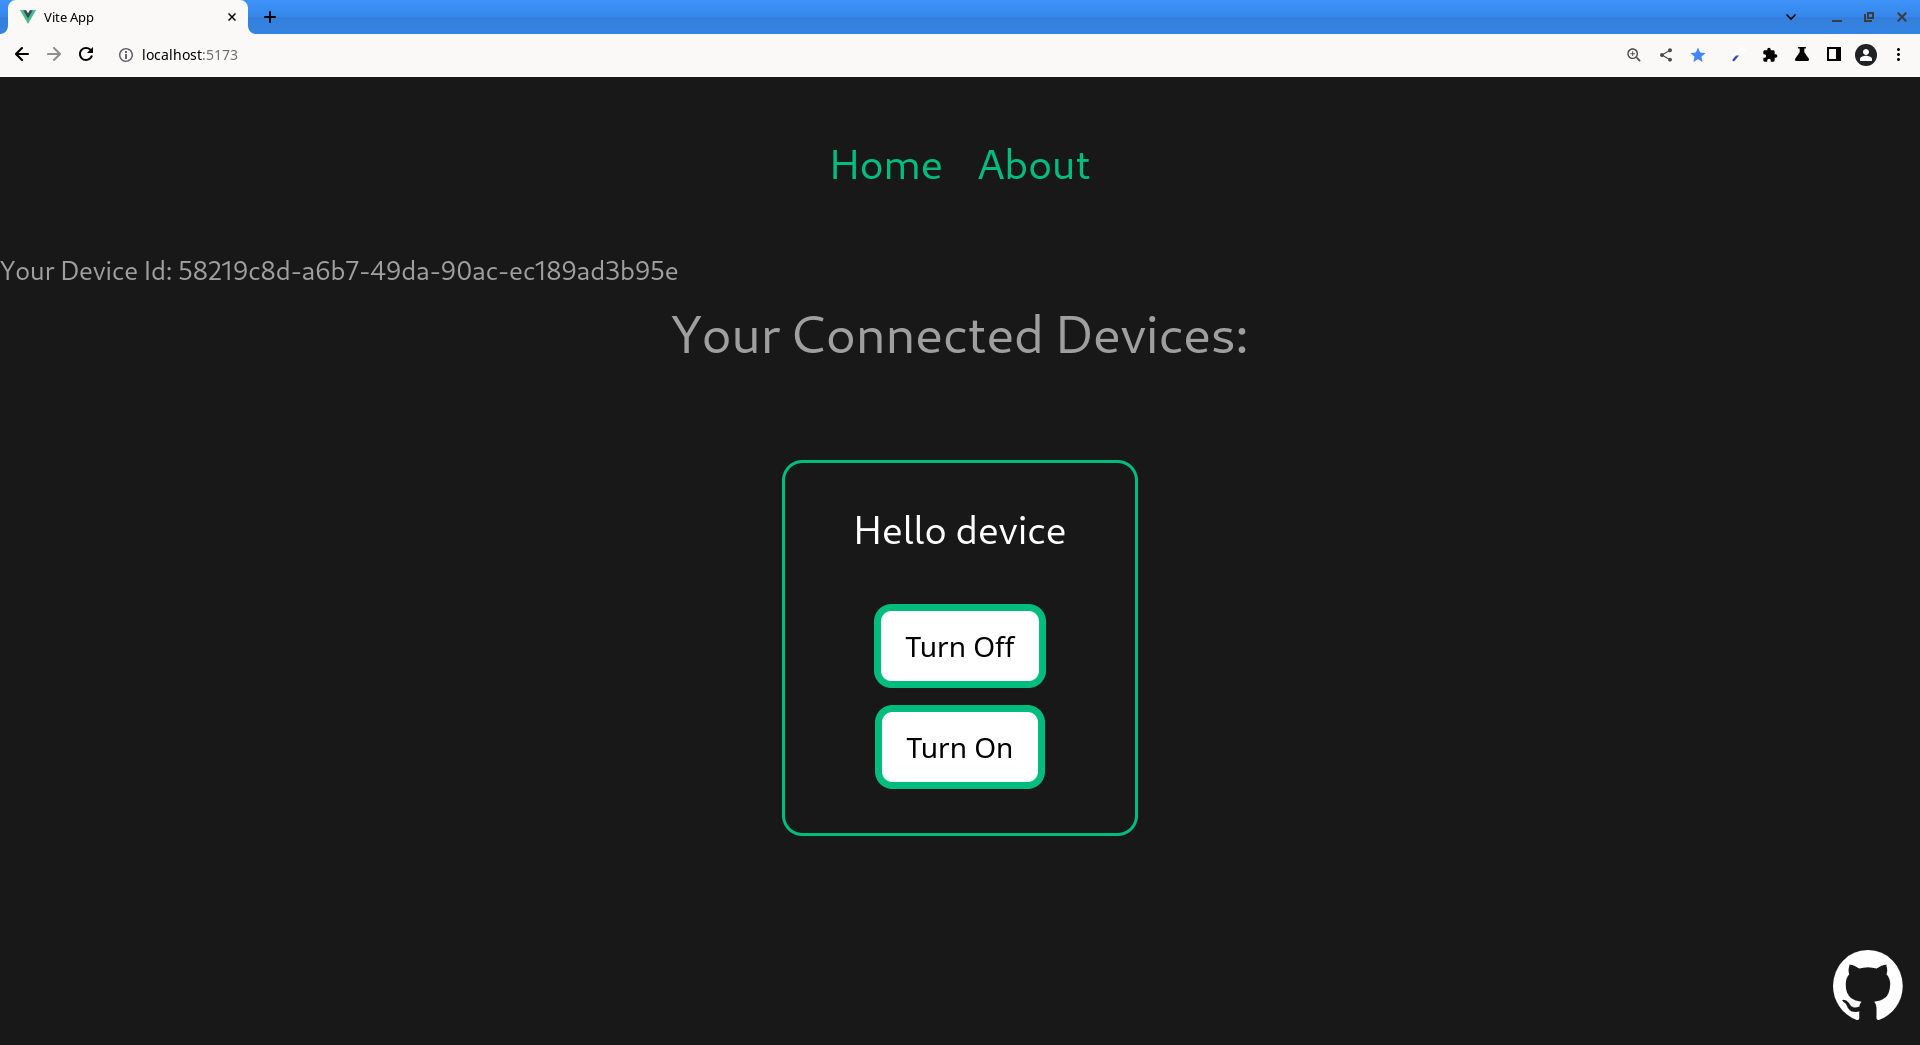
\includegraphics[width=\textwidth]{testing_web_frontend_one_device}
\label{fig:web_frontend_one_connected_device}
\end{figure}





\subsection{Running with One connected Device over Wifi} 
\subsection{Running with multiple connected devices}
\subsection{Sending incorrect signatures}
\section{Performance Testing}
